\subsection{Polynomials and the Affine Space} 

Variables considered per default in algebra are \textit{formal variables (symbols)}. Formal means roughly placeholder for anything. There is no domain attached to this. 

Formal variables are used in \textit{formal expressions (symbolic expressions)}. 

\textbf{Note the difference to functions}: Symbolic expressions are just expressions, not functions. In particular, they \hspace*{5.2cm}don't have any domain or co-domain.  \\

In what follows, we consider $n$ formal variables ($n \in \mathbb{Z}_{>0}$) whose default names will be $x_1, \ldots, x_n$.  For $n=1$, it is customary to use $x$, If $n=2$ it's cosumary to use $x$ and $y$. For $n = 3$ it's cosumary to use $x, y, z$. 

\begin{definition}[title = Definition 1.1.1] 
    Let $x = (x_1, \dots, x_n)$ be the vector of $n$ formal variables and $\alpha = (\alpha_1, \dots, \alpha_n) \in \mathbb{Z}_{\geq 0}^n$ a vector of $n$ non-negative integers. Then the expression 
    \[x^{\alpha} := x_1^{\alpha_1} \cdot \ldots \cdot x_n^{\alpha_n}\] 
    is called the \textit{monomial for the expotent vector $\alpha$}.  $\alpha_1 + \ldots + \alpha_n$ is called the \textit{(total) degree of the monomial $x^{\alpha}$}, denoted as $|\alpha|$. \\[0.3em] 
    Our \textit{coefficient domain} will be an arbitrary field which we denote by $k$ thoughout.
\end{definition}

\clearpage

\begin{example}
    Given: $x^{(2, 3)} = x_1^2 \cdot x_2^3 \text{ and } x^{(3, 0)} = x_1^3$ 
    \begin{center}
        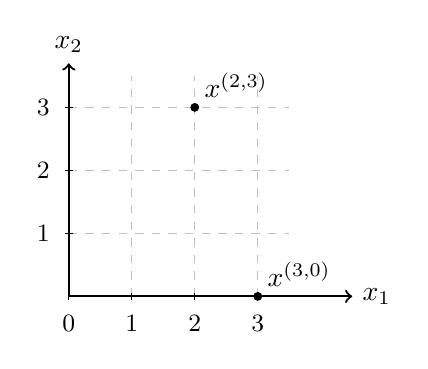
\begin{tikzpicture}[scale=0.8]
        \foreach \value in {1,2,3} {
          \draw[dashed, gray!50] (\value,0) -- (\value,3.5);
          \draw[dashed, gray!50] (0,\value) -- (3.5,\value);
        }
        \draw[->, thick] (0,0) -- (4.5,0) node[right] {$x_1$};
        \draw[->, thick] (0,0) -- (0,3.7) node[above] {$x_2$};
        \foreach \value in {0,1,2,3}
          \draw (\value,0.06) -- (\value,-0.06)
            node[below=2pt] {\small $\value$};
        \foreach \value in {1,2,3}
          \draw (0.06,\value) -- (-0.06,\value)
            node[left=2pt] {\small $\value$};
        \fill (2,3) circle (2pt) node[above right] {$x^{(2,3)}$};
        \fill (3,0) circle (2pt) node[above right] {$x^{(3,0)}$};
        \end{tikzpicture}
    \end{center}
\end{example}

You already know some fields: $\mathbb{Q}, \mathbb{R}, \mathbb{C}\mathbb{F}_p$ and $\mathbb{F}_{p^N}$ where $p$ is prime, $\mathbb{Q}[\sqrt{2}]$ 

\hspace*{0.5cm} $\rightarrow$ It's important to know some examples of them. 

\begin{definition}[title = Definition 1.1.2] 
    A \textit{polynomial in variables $x_1, \dots, x_n$} with coefficients in $k$ is a formal expression of the form 
    \begin{equation}
        f = \sum_\alpha c_\alpha x^\alpha, 
    \end{equation}
    where $\alpha$ runs over $\mathbb{Z}_{\geq 0}^n$ and $c_\alpha \neq 0$ for any finitely many choices of $k$. \\

    \hspace*{0.5cm}\textcolor{airforceblue}{\textit{(You must have seen polynomials in one variable before... surprise, surprise - life is not one-dimensional!)}}  \\

    $c_\alpha x^\alpha$ (when $c_\alpha \neq 0$) is called a \textit{term of degree} $|\alpha|$ of $f$. The \textit{(total) degree of $f$} is the maximum degree of the terms in $f$: \[\deg f = \max\{|\alpha|: \alpha \in \mathbb{Z}_{\geq 0}^n, c_\alpha \neq 0\}\]
    
    The \textit{zero polynomial} $f =0$ has no terms and by this degree $-\infty$.  
    
    The \textit{set of all polynomials in $x_1, \dots, x_n$} with coefficients in $k$ is denoted by $k[x_1, \dots, x_n]$. \\
    
\begin{center}
  \textcolor{gray}{------------------------------------------- 06.10.2026 --------------------------------------------} \\[0.3em]
\end{center} 

    \textbf{Note:} Polynomials are formal expressions, not functions. \\[0.7em]
    Equality of two polynomials is \underline{defined} through comparison of coefficients. \\[0.5em]
    We make $k[x_1, \dots, x_n]$ an algebraic structure by introducing the basic operations, which are the addition and the multiplication. \\

    \textbf{Addition:} \[\sum_\alpha c_\alpha \cdot x^\alpha + \sum_\alpha d_\alpha \cdot x^\alpha := \sum_\alpha (c_\alpha + d_\alpha) \cdot x^\alpha\] 
    \textbf{Multiplication:} \[\left(\sum_\alpha c_\alpha \cdot x^\alpha\right) \left(\sum_\beta d_\beta \cdot x^\beta\right) := \sum_{\alpha, \beta} c_\alpha \cdot d_\beta \cdot x^{\alpha + \beta} = \sum_\gamma \left(\sum_{\alpha, \beta: \alpha + \beta = \gamma} c_\alpha \cdot d_\beta \right) \cdot x^\gamma\]
  \end{definition} 
\clearpage

\begin{remark}[title=Adrian's Question]
Adrian asked about the role of the condition $c_\alpha \ne 0$ for finitely many $\alpha$. It makes the number of terms finite and allows one to define evaluation of polynomials later on. But: if one remove the 
finiteness assumption, what one gets is the notion of a formal power series. The set of all formal power series with coefficients in $k$ and variables $x_1,\ldots,x_n$ is denoted as $k[[x_1,\ldots,x_n]]$. They 
have applications in different situations, including combinatorics (generating functions). 
\end{remark} 

\begin{remark}[title = Remark 1.1.3] 
    We can view $k$ as a subset of $k[x_1, \dots, x_n]$ and by this $k[x_1, \dots, x_n]$ contains $1\in k$ (The multiplecative identity). 

    It turns out that $(k[x_1, \dots, x_n], +, \cdot)$ is a unitary, commutative ring:   

    \begin{minipage}[t]{0.33\textwidth}
      \begin{align*}
          f+(h+g) &= (f+h)+g \\
          f+g &= g+f \\
          f + 0 & = f\\ 
          f + (-f) & = 0  
      \end{align*}
    \end{minipage}
    \begin{minipage}[t]{0.33\textwidth}
      \begin{align*}
          f \cdot (h \cdot g) &= (f \cdot h) \cdot g \\
          f \cdot g &= g \cdot f \\
          f \cdot 1 & = f\\ 
      \end{align*} 
    \end{minipage}
    \begin{minipage}[t]{0.33\textwidth}
      \begin{align*}
          (f + g) \cdot h & = f \cdot h + g \cdot h
      \end{align*}
    \end{minipage}

    This holds for all $f, g, h \in k[x_1, \dots, x_n]$. The $-f$ is the unique polynomial whose addition to $f$ gives 0.
\end{remark}

\begin{remark}[title = Remark 1.1.4]
    There are three basic choices of n:  
    \begin{center}
    \begin{tabular}{l|l|l}
      n = 1 & $x_1$ & x \\
      n = 2 & $x_1, x_2$ & x, y \\
      n = 3 & $x_1, x_2, x_3$ & x, y, z
    \end{tabular} 
  \end{center} 

    Later, a connection to geometry will be established. These three basic cases will get connected to line resp. plane and resp. 3-dim. space.
\end{remark}

\begin{definition}[title = Definition 1.1.5]
    In algebraic geometry, the space $k^n$ of all $n$-tuples with the coefficients in $k$ is called the \textit{$n$-dimentional affine space over the field $k$}.  
    
    From linear algebra we know, that $k^n$ is a $k$-vector space.  
\end{definition} 

\textbf{Fun Fact:} It's by far not the only space one can consider. Another very common and important space is the projective space. Actually, in the Elliptic Curve Cryptography (ECC), 
the elliptic curve is considered in the projective space.

\begin{definition}[title = Definition 1.1.6]
    We can evaluate $f = \sum_\alpha c_\alpha \cdot x^\alpha \in k[x_1, \dots, x_n]$ at a point $(a1, \dots, a_n) \in k^n$ of the affine space obtaining the value. 
    \[f(a_1, \dots, a_n) = \sum_{\alpha = (\alpha_1, \dots, \alpha_n)} c_\alpha a_1^{\alpha_1} \cdots a_n^{\alpha_n}\]    
  
    This gives rise to to a function $k^n \to k$. This function is usually denoted again by $f$, even though $f \in k[x_1, \dots, x_n]$ and $f: k^n \to k$ is not the 
    same thing. In math, such a situation is called abuse of notation. 
    
    \hspace*{0.5cm}\textcolor{airforceblue}{\textit{I know it's not quite right, but I know what I'm doing}}
    
    Functions arising this way are called \textit{polynomial functions}.
\end{definition} 

\begin{remark}[title = Remark 1.1.7]
    In some fields, for example, in finite fields $k$, different polynomials in $k[x_1, \dots, x_n]$ may define the same polynomial function.
\end{remark} 

\clearpage
\begin{example}[title = Example]
Consider the finite field $\mathbb{F}_{2} = \{0, 1\}$ with 
\begin{tabular}{c| c c}
    + & 0 & 1 \\
    \hline
    0 & 0 & 1 \\
    1 & 1 & 0
\end{tabular}
and 
\begin{tabular}{c| c c}
    $\cdot$ & 0 & 1 \\
    \hline
    0 & 0 & 0 \\
    1 & 0 & 1
\end{tabular}

\vspace{0.3em} 

\begin{minipage}[t]{0.33\textwidth}
    $f = x^2 + x \in \mathbb{F}_2[x]$ \\
    $g = x^3 + x \in \mathbb{F}_2[x]$
\end{minipage}
\begin{minipage}[t]{0.33\textwidth}
  $f : \mathbb{F}_2 \to \mathbb{F}_2$

  \begin{tabular}{c |c}
    $a \in \mathbb{F}_2$ & $f(a) \in \mathbb{F}_2$ \\
    \hline
    0 & 0 \\
    0 & 0 
  \end{tabular}
\end{minipage}
\begin{minipage}[t]{0.33\textwidth}
  $g : \mathbb{F}_2 \to \mathbb{F}_2$

  \begin{tabular}{c |c}
    $a \in \mathbb{F}_2$ & $g(a) \in \mathbb{F}_2$ \\
    \hline
    0 & 0 \\
    0 & 0 
  \end{tabular}
\end{minipage}

So, both functions are the same, but the polynomials are different 
\end{example}

\textbf{Fun Fact:} Do we need $\mathbb{F}_2[x]$ for anything? \\
$\rightarrow$ Yes! Advanced Encryption Standard (AES) used the field $\mathbb{F}_{256}$, whose construction requires taking a polynomial from $\mathbb{F}_2[x]$.  

 
  \begin{center}
    \textcolor{gray}{------------------------------------------- 12.10.2026 --------------------------------------------} \\[0.3em]
  \end{center} \ \\[0.15em]  
  \textbf{Note:} Test today $\rightarrow$ some will need to catch up \\
   $\rightarrow$ Check-In Date for the catch-up cohort: $9^{th}$ of November, you show your progress on the form of the written 
  solutions of the exercises from a textbook (linear algebra over arbitrary fields, with proofs). 
  
\begin{exercise}[title = Entry Level Exercise]
  \begin{enumerate}
    \item Formulate mathematical induction (with words and/or formulas).  
    \item Define the notion of a group. Give an example of an abelian and a non-abelian group. 
    \item Define the notion of a ring. Give an example of a commutative and a non-commutative ring. 
    \item Define the notion of a field. Give an example of an infinite and finite field. 
    \item Let $k$ be a infinite field and consider a univariate polynom $f \in k[x]$. \\ 
    Proof: $f = 0$ $\Leftrightarrow$ $f(a) = 0, \forall a \in k$. 
  \end{enumerate}
\end{exercise} 

  \begin{center}
    \textcolor{gray}{------------------------------------------- 13.10.2026 --------------------------------------------} \\[0.3em]
  \end{center} 
  \vspace{0.5cm}
\begin{theorem}[title =Theorem 1.1.8]
  Let the field $k$ be infinite. Then $f \in k[x_1, \dots, x_n]$ is a zero polynomial (all coefficients of $f$ are zero) if and only if $f: k^n \to k$ is a zero function. 
  
  \paragraph{Proof:} The implikation ($\Rightarrow$) is trivial because $f = \sum_{\alpha} c_{\alpha} x^{\alpha}$ gets evaluated to zero on $k^n$ when all of the $c_{\alpha}$'s are zero. 
  So, the actual work is to show the converse $(\Leftarrow)$. For the converse, we are going to use the mathematical induction on $n$. \\
  
  We consider the case $n = 1$. as a basis of the induction. We consider a polynomial $f$ in one variable $x$, which is \underline{not} a zero polynomial 
  and show that $f(a) \neq 0$ for some $a \in k$. We can write $f$ as $f = \sum_{i=1}^{d} c_i x^i$ where $d \in \mathbb{N}_0$ and $c_d \neq 0$.  \\
  
  \begin{addmargin}[0.6cm]{0cm}  
    \textbf{Version 1 of the argument:} \hspace*{0.2cm} Pick a zero of $f$, as long as there is one, let's call it $a_1 \in k$ and divide $f$ by $(x - a_1)$ (in the sense of long division). 
    It get's divided with the 0 remainder. So, we have $f = (x = a_1) \cdot g$ where $g$ has degree $d-1$ (the degree drops). If $g$ is divisible by $(x - a_1)$, keep dividing. 
    Once this process of dividing by $(x - a_1)$ is finished, we have $f = (x - a_1)^{p_1} \cdot h(x)$, where the degreee of $h$ is smaller than the degree of $g$ and $a_1$ is not a zero of $h$. 
    If there is another zero, say $a_2 \in k$, do the same obtaining  $f = (x - a1)^{p_1} \cdot (x - a_2)^{p_2} \cdot u(x)$, where $a_1$ and $a_2$ are both not zero of $u(x)$. 
    Iterating this way, we end up at the representation $f = (x - a_1)^{p_1} \cdot (x - a_2)^{p_2} \cdot \dots \cdot (x - a_m)^{p_m} \cdot w(x)$ where $a_1, \ldots, a_m \in k$, $deg f = p_1 + \ldots + p_m + deg(w)$ 
    and $w$ has no zero in $k$. This shows that a non-zero polynomial of degree $d \in \mathbb{N}_0$ with at most $d \in \mathbb{N}_0$ zeros, where $d$ is finite, but 
    our field $k$ is infinite. So, $f : k \to k$ is only zero on $\{a_1, \ldots, a_m\}$ and so it's not a zero function.
  \end{addmargin}


\end{theorem}
\clearpage
  \begin{theorem}[title =Theorem 1.1.8 (Continued)]
    \begin{addmargin}[0.6cm]{0cm}  
    \textbf{Version 2 of the argument for $n = 2$:} \hspace*{0.2cm} Let's use linear algebra and polynomial interpolation. Let's consider all polynomial of degree at most $d \in \mathbb{N}$, 
    where $d$ is fixed and arbitrary. Denote the set of these polynomials by $k[x]_d = \{\sum_{i = 0}^{d} c_i x^i: c_i \in k \text{for every} i\}$. 
    This is a $k$-vector space of dimension of $d + 1$.  
    We fix $d + 1$ dstinct values $a_1, \ldots, a_{d+1}$ in $k$ (our field is infinite, so no matter how large our $d$ is, we always have  such a choice) 
    and consider the linear map that evaluates $f \in k[x]_d$ at these values. 
    \[ev(f) = (f(a_1), \ldots, f(a_{d+1}))\] 

    \begin{minipage}{0.49\textwidth}
    This is the map $ev: \underbrace{k[x]_d}_{\text{dimension } d+1} \to \underbrace{k^{d + 1}}_{\text{dimension } d+1}$.  \\
    
    We're going to show that this map is surjective (in the language of the numerical mathematics: the polynomial interpolation task is solvable).  
    \end{minipage}
\hspace*{0.2cm}
    \begin{minipage}{0.49\textwidth}
    \begin{tikzpicture}[>=stealth, scale = 0.8]
        % x-Achse
        \draw[->] (-0.5,0) -- (6.5,0) node[right] {$x$};

        % Parabel (nach oben verschoben)
        \draw[green!60!black, thick, domain=0.3:5.7, smooth, samples=100]
          plot (\x, {0.25*(\x-3)^2 + 2});

        % Markierungen, gestrichelte Linien und Punkte
        \foreach \x/\l in {1/1, 3/2, 5/3} {
          \draw (\x,0.08) -- (\x,-0.08) node[below] {$x_{\l}$};
          \draw[dashed] (\x,0) -- (\x,{0.25*(\x-3)^2 + 2});
          \fill (\x,{0.25*(\x-3)^2 + 2}) circle (2.5pt);
        }
    \end{tikzpicture}
  \end{minipage}

  Let's fix an arbitrary $y = (y_1, \ldots, y_{d+1}) \in k^{d + 1}$ and determine an $f \in k[x]_{d+1}$ satisfying $f(a_i) = y_i$ for all $i \in \{1, \ldots, d+1\}$.   

  Introduce \[l_i(x) = \prod_{j = 1 \ldots, d+ 1: j \neq i} \frac{x - a_j}{a_i - a_j} \in k[x]_{d}\] which satisfies 
  \[l_i(a_j) = \begin{cases}
    1, & \text{if } i = j \\ 
    0, & \text{if } i \neq j
  \end{cases}\]
  Now, it is clear that $f = y_1 \cdot l_1 + \ldots y_{d+1} \cdot l_{d+1}$ satisfies $f(a_i) = y_i$ for all $i = 1, \ldots, d+1$. 
  We have shown that $ev: k[x]_d \to k^{d+1}$ is surjective. So, from linear algebra, we know that $f$ is also injective so that only the zero polynomial 
  is mapped to $(0, \ldots, 0)$ by $ev$. 
\end{addmargin} \ \\
If you like more details on that point:  by the rank-nullity theorem, \[\underbrace{\dim \text{im}(ev)}_{\text{dimension} d+1}  + \underbrace{\dim \ker(ev)}_{\text{dimension} d+1} = \dim k[x]_d,\] so that $\dim \ker(ev) = 0$. \\

  We have done the case $n =1$ and we continue with the inductive argument. Assume that the assertion is already verified for polynomials in $n -1$ variables for some $n \geq 2$. 
  Based on this, we verify the assertion for polynomials in $n$ variables. \\
    \begin{addmargin}[0.6cm]{0cm}  

  We can write a polynomial $f \in k[x_1, \dots, x_n]$ as an element of $k[x_1, \dots, x_{n-1}][x_n]$, so we write $f= \sum_{i = 1}^{d} g_i(x_1, \dots, x_{n-1}) \cdot x_n^i$ with $g_1, \ldots, g_d  k[x_1, \dots, x_{n-1}]$. 
  We fix arbitrary values for $x_1, \ldots, x_{n-1}$, which we denote by $a_1, \ldots, a_{n-1} \in k$. Fixing these values, we get $f(a_1, \ldots, a_{n-1}, x_n) = \sum_{i=1}^{d}g_i(a_1, \ldots, a_{n-1}) \cdot x_n^i \in k[x_n]$. 
  By the $n=1$ case of our argument, whenever $f(a_1, \ldots, a_{n-1}, x_n)$ defines the zero function $k \to k$, it is a zero polynomial. 
  Hence, its coefficients $g_i(a_1, \ldots, a_{n-1})$ are a;; zero. But since $(a_1, \ldots, a_{n-1})$ are \underline{arbitrary} values from $k$, the induction assumption implies that $g_i(x_1, \ldots, x_{n-1})$
  is also a zero polynomial. Consequently, $f$ is a zero polynomial.   
    \end{addmargin}
  \begin{flushright}
    $\Box $
  \end{flushright}
\end{theorem} 

\clearpage

\begin{center}
    \textcolor{gray}{------------------------------------------- 19.10.2026 --------------------------------------------} \\[0.3em]
\end{center} 
\vspace{0.5cm} 

\begin{corollary}[title = Corollary 1.1.9]
  Let the field $k$ be infinite. Then two polynomials $f,g \in k[x_1, \dots, x_n]$ are equal if and only if there respective polynomial functions $f, g:k^n \to k$ are equal. 
  \paragraph{Proof:}By 1.1.8 the difference function $f -g: k^N \to k$ is a zero function if and only if $f - g$ is a zero polynomial. This immediately gives the assertion. 
  
  \begin{flushright}
    $\Box $
  \end{flushright}
\end{corollary}

\textbf{Fun Fact:} There is also a multivariatte polynomial interpolation, which is even more fun than the univariat and helps in this case.

\begin{definition}[title = Definition 1.1.10]
  A field $k$ is called \textit{algebraically closed} if for every polynomial $f \in k[x]$ of degree $\geq 1$ there exists an $a \in k$ such that $f(a) =0$. 
  
  (That is, each univariat polynomial equation over $k$ of degree $\geq 1$ has a solution in $k$.) 
\end{definition}

\begin{theorem}[title = Theorem 1.1.11]
  The field $\mathbb{C}$ of complex numbers is algebraically closed. 

  (This result is called the fundamental theorem of algebra and we don't prove is here.)  
\end{theorem} 

\begin{exercise}[title = Small Exercise 1.1.11a] 
  Let $k$ a finite field. Show that $k$ is not algebraically closed. 
  \paragraph{Solution:} 
  \begin{itemize}
    \item \textbf{Leo:} $k = \{k_1, \ldots, k_n\}$ and $f = (k_1 - x)\cdot(k_2 -x) \dots + k_1$, where $k_1 \neq 0$ 
    \item \textbf{Prof. Averkov:} \[f = \prod_{s \in k}(x -s) + 1\]
    $f(a) = 1$ for all $a \in k$ by construction. The degree of $f$ is $deg f = |k| \geq 2 \geq 1$. 
  \end{itemize} \ \\

  \textbf{Add On:} Let's take the field $\mathbb{Z} = \mathbb{F}_2$. Please write down this polynomial for this particular field. (Expand brackets) 
  \paragraph{Solution:} 
  \[
    f = \prod_{s \in k}(x -s) + 1 = (x -1) \cdot (x -0) + 1  = (x +1) \cdot x + 1 = x^2 + x + 1
   \]
   This polynomial will help you to create another finite field. 
\end{exercise} 

